\chapter{Surrogate Assessment and Macroscopic Application}\label{ch:assessment}

This chapter evaluates whether the trained surrogate reproduces the direct RVE
solutions and whether it can be used in a macroscopic simulation. After the
comparison with the proposal and the committee's recommendations, the RVE is checked
against micromechanics, the training and test performance of the surrogate are
presented, and its errors are analysed separately for volumetric and deviatoric
response.

\section{Proposal goals and their achievement}

{\small
\begin{xltabular}{\textwidth}{@{}p{3.6cm}p{2.3cm}X@{}}
\caption{Milestones of the proposal and their outcome.}\label{tab:proposal}\\
\toprule
Proposal item & Status & Outcome / justification\\
\midrule
\endfirsthead
\caption[]{\emph{(continued)}}\\
\toprule
Proposal item & Status & Outcome / justification\\
\midrule
\endhead
\bottomrule
\endfoot
M1 Environment, repository, periodic RVE, kinematic check (target $<10^{-12}$) &
  achieved & Native periodic spaces; P2-V1 jump $2.2\times10^{-16}$.\\
M2 Hill--Mandel averaging, data over $\vfrac$ (target: energy deviation $<1\,\%$) &
  achieved, exceeded & Reaction-based stress; P2-V5 $1.2\times10^{-15}$; ten datasets with 4653 distinct direct-RVE records.\\
Rigid glass via stiffness penalty & replaced & Exact rigid trace with free rotation (no penalty parameter, no particle deformation).\\
RVE tangent by forward differences & replaced & Exact Schur condensation, Taylor order $2.000$ (P2-V6); differences used only for checks.\\
M3 pICNN, softplus weights, normalization, Sobolev loss & implemented; accuracy \emph{not} achieved in shear &
  Polyconvex architecture verified (S-V1); normalization corrected to an objective form; deviatoric accuracy is limited by loss scaling (\cref{sec:diagnosis}).\\
pICNN inputs $\mathcal N(I_1,I_2,\vfrac)$ & extended & Features $[I_1,I_2,J,-\ln J]$ plus $\vfrac$ context; $J$ is needed for the compressible volumetric response and the stress-free normalization.\\
Sobolev loss with $\lambda_A\gg\lambda_\Psi$ (tangent prioritized) & \emph{not} followed &
  Implemented weights $w_\Psi=1$, $w_P=1$, $w_A=0.1$ on a relative-Frobenius tangent term (\cref{eq:loss}); the tangent was not prioritized, and its relative norm is itself volumetric-dominated (\cref{sec:diagnosis}).\\
V3: FD error ``drops to machine precision at $\epsilon\to10^{-7}$'' & corrected expectation &
  Not attainable: V3 shows the truncation/round-off V-curve with minimum $2.3\times10^{-10}$ near $\epsilon=10^{-6}$; FD is used only as a check.\\
V4 on a single hexahedral element & changed &
  V4 uses a coarse tetrahedral cube mesh; single-hexahedron tests are V0d/V0e, V7 and V8.\\
Material data $\mu_\mathrm{PDMS}\approx2\,$MPa, $E_\mathrm{glass}\approx70\,$GPa & idealized &
  Dimensionless $\mu=1$, $\kappa=10^4$; glass exactly rigid (no $E_\mathrm{glass}$ needed); no calibration to measured PDMS.\\
M1 continuous-integration pipeline & achieved &
  GitHub Actions workflow and the runner \code{run\_tests.sh}, in addition to manual and PBS test runs.\\
AI tools ``strictly'' for syntax, plotting templates, NumPy & broader use &
  Also used for understanding theory and libraries, discussing code structure and
  errors, test cases, PBS scripts and writing support (\cref{ch:chatbots}).\\
M4 AD tangent, $6\times6$ Voigt mapping, FD check & achieved, corrected & Full $9\times9$ tangent instead of $6\times6$; V3 minimum error $2.3\times10^{-10}$.\\
M5 Macroscopic BVP, custom Newton, manual assembly & achieved & Bridge with globalized Newton; macro tangent check $6.5\times10^{-10}$ (M-V0).\\
M6 Single-element benchmark (quadratic convergence) and multi-element component (dogbone) &
  partly achieved & V4 quadratic; clamped-cube component instead of a dogbone; $P_1$ reaches $5\,\%$ but is locked; $P_2$ reaches $1\,\%$ on two of three meshes (\cref{sec:macro}).\\
M7 Documentation, README per test, defense & achieved & Manual in \cref{ch:manual}; \code{tests\slash{}README.md} lists command, inputs and expected result of every test.\\
\end{xltabular}
}

\paragraph{Additional work beyond the proposal.} The following studies were not
promised and were carried out in addition, all with the frozen checkpoint: the
30-case timing benchmark (\cref{ch:performance}), the loading-path sweep, the
volume-fraction map, inverse design of $\vfrac$, the cell-orientation (isotropy)
audit, the small-strain micromechanics comparison, and the sampled acoustic-tensor
screen. The shear-adaptation study belongs to the main scope as a corrective step.

\section{Response to the committee's recommendations}\label{sec:committee}

After the proposal defense, the committee (Dr.\ S.\ Pr\"uger) asked first for a
proof of concept of the pICNN, including stress and tangent, inside NGSolve, and
only then for RVE data generation. It also raised several technical questions.
\Cref{tab:committee} lists each point and where the report answers it.

{\small
\begin{xltabular}{\textwidth}{@{}p{5.0cm}X@{}}
\caption{Committee recommendations and their implementation.}\label{tab:committee}\\
\toprule
Recommendation / question & Response in this project\\
\midrule
\endfirsthead
\caption[]{\emph{(continued)}}\\
\toprule
Recommendation / question & Response in this project\\
\midrule
\endhead
\bottomrule
\endfoot
Proof of concept first: pICNN with stress and tangent in NGSolve, trained on neo-Hookean data, before extensive data generation; establish with PyTorch what the TensorFlow tutorial shows &
  Phase~1 (\cref{sec:bridge}). The network is trained on the neo-Hookean law; the data
  are homogeneous states, so a single element under affine displacement reproduces
  them exactly. It is coupled through quadrature-point spaces to an NGSolve Newton
  solver and verified by V1--V6 and V0d before any RVE campaign.
  The TensorFlow tutorial and the closer NGSolve forum example are compared in
  \cref{tab:available}.\\
How are rigid inclusions handled? &
  No stiff phase: the cavity surface carries the exact rigid map \cref{eq:rigid};
  the rotation follows from moment equilibrium (P2-V2, P2-V7).\\
Periodicity through periodic function spaces on a periodic mesh &
  Implemented with Netgen face identification and NGSolve \code{Periodic} spaces;
  the custom ``PBC enforcer'' of the proposal was dropped (P2-V1).\\
How is the overall tangent computed? &
  Exact Schur condensation of the energy Hessian \cref{eq:schur}; Taylor order
  $2.000$ (P2-V6).\\
Macroscopic weak form: which fields, FE$^2$, or a mixed formulation for incompressibility? &
  Offline homogenization, not FE$^2$; the macro problem has displacements only. The
  locking analysis (\cref{sec:macro}) confirms the committee's concern: a mixed
  $u$--$p$ macro formulation is required for meaningful component responses.\\
The macro BVP is not ``driven by PyTorch'' &
  Wording corrected: NGSolve applies the boundary conditions and solves for the
  displacement; PyTorch only evaluates the constitutive law (\cref{sec:macro-method}).\\
Volumetric locking depends on the element choice &
  RVE: Taylor--Hood $P_2/P_1$ mixed formulation (P2-V3). Macro scale: locking of
  $P_1$ demonstrated quantitatively (\cref{tab:macro}).\\
Finite-difference tangent: choice of $\epsilon$ and attainable accuracy &
  FD is no longer used for any production tangent. V3 shows the expected
  truncation/round-off V-curve with a minimum error of $2.3\times10^{-10}$ near
  $\epsilon=10^{-6}$, so machine precision is \emph{not} reached by FD.\\
\end{xltabular}
}

\section{Physical plausibility of the RVE: small-strain moduli}

Before any surrogate is judged, its reference must be credible. Projecting the
direct-RVE tangent at $\Fbar=\Iten$ onto one volumetric and five orthonormal
deviatoric modes gives $K_{\mathrm{eff}}$ and $\mu_{\mathrm{eff}}$
(\cref{tab:moduli}, \cref{fig:moduli}). They lie within $0.2$--$1.1\,\%$ (bulk) and
$0.25$--$0.83\,\%$ (shear) of the Mori--Tanaka estimate \cref{eq:mt}, slightly
below it. The deviatoric anisotropy of the cubic cell grows from $0.2\,\%$ to
$4.1\,\%$ with $\vfrac$. This is the expected signature of one particle per cubic
cell, and it explains why the small deficit is not a bound violation. Rotating the
cell by three non-cubic rotations changed the energy and stress by at most
$5.6\times10^{-5}$ and $2.8\times10^{-5}$ (relative), which supports the isotropy
assumption of the surrogate within the tested states. The direct RVE is
therefore a sound reference.

\begin{table}[htbp]
\centering\small
\caption[Small-strain moduli ($\mu=1$, $\kappa=10^4$)]{Small-strain moduli ($\mu=1$, $\kappa=10^4$). The pICNN values of both checkpoints are computed directly from the network Hessian at $\F=\Iten$.}
\label{tab:moduli}
\begin{tabular}{@{}lccccccc@{}}
\toprule
& \multicolumn{3}{c}{$\mu_{\mathrm{eff}}$} & & \multicolumn{3}{c}{$K_{\mathrm{eff}}/10^4$}\\
\cmidrule{2-4}\cmidrule{6-8}
$\vfrac$ & 0.02 & 0.05 & 0.10 && 0.02 & 0.05 & 0.10\\
\midrule
Mori--Tanaka & 1.051 & 1.132 & 1.278 && 1.0204 & 1.0526 & 1.1111\\
direct RVE & 1.048 & 1.124 & 1.267 && 1.0185 & 1.0469 & 1.0988\\
pICNN frozen & 1.526 & 1.731 & 2.147 && 1.0231 & 1.0361 & 1.0873\\
pICNN shear-adapted & 1.349 & 1.527 & 1.892 && 1.0167 & 1.0478 & 1.0941\\
\midrule
frozen vs.\ RVE & $+45.6\,\%$ & $+54.0\,\%$ & $+69.5\,\%$ && $+0.4\,\%$ & $-1.0\,\%$ & $-1.0\,\%$\\
\bottomrule
\end{tabular}
\end{table}

\begin{figure}[htbp]
\centering
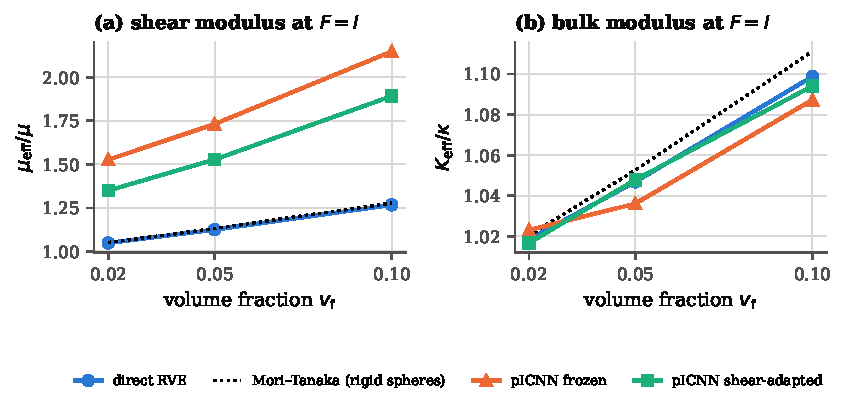
\includegraphics[width=\textwidth]{fig_small_strain_moduli.pdf}
\caption[Effective moduli at $\F=\Iten$]{Effective moduli at $\F=\Iten$. The direct RVE follows the Mori--Tanaka
estimate. Both surrogates reproduce the bulk modulus but overestimate the shear
modulus, by $46$--$70\,\%$ (frozen) and $29$--$49\,\%$ (shear-adapted).}
\label{fig:moduli}
\end{figure}

\paragraph{Inference.} The direct RVE is a credible reference: it reproduces the bulk and shear moduli of a rigid-sphere
composite to better than $1.2\,\%$ and is slightly softer than the Mori--Tanaka estimate, as expected
for a cubic arrangement. The surrogate inherits the correct bulk response but not the shear
response, so the shear error found later is a property of the surrogate, not of its labels.

\section{Training and test performance}\label{sec:trainperf}

\Cref{fig:training} shows the loss histories. The Phase~1 network trained on
neo-Hookean data decreases the loss by three orders of magnitude
(\cref{fig:training}a). On the RVE data, training and validation losses decrease
together by five orders of magnitude in the first stage (\cref{fig:training}b), and
continue to decrease slowly during the fine-tune on the combined Phase~6/7 data
(\cref{fig:training}c). Validation and training losses remain close throughout, so
there is no sign of overfitting; the oscillations reflect the small batch size and the
stochastic tangent sub-batch. The checkpoint with the lowest validation loss
(epoch~2750) was frozen.

\begin{figure}[htbp]
\centering
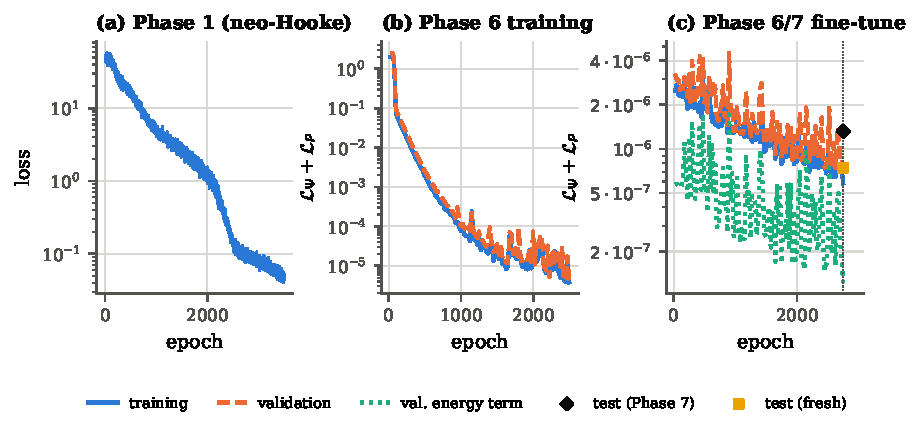
\includegraphics[width=\textwidth]{fig_training_curves.pdf}
\caption[Training histories]{Training histories. (a) Phase~1 network on neo-Hookean data. (b) First
training stage on the Phase~6 RVE data. (c) Fine-tune on Phase~6/7 data, with the
selected epoch (dotted line) and the losses of the frozen checkpoint on the two test
sets. Loss: energy and stress terms of \cref{eq:loss}, in normalized units.}
\label{fig:training}
\end{figure}

\Cref{tab:testloss} compares the losses of the frozen checkpoint on the training,
validation and test data. The test sets were not used for the gradient updates or the epoch selection of the stage in
which they are evaluated, but they are not all independent: the Phase~7 test split was
also evaluated with the stage-1 checkpoint, and 66 of the 600 Phase~7 records entered the
stage-2 training and validation sets. Only the fresh holdout of 90 records, generated after
the checkpoint was frozen, is fully independent.
The Phase~7 test split (531 states) and a fresh holdout of newly generated RVE
states (72 states) give energy-plus-stress losses of the same order as the training
loss ($1.3\times10^{-6}$ and $7.5\times10^{-7}$ against $5.8\times10^{-7}$). The model
therefore generalizes to unseen deformation states within the training envelope.

\begin{table}[htbp]
\centering\small
\caption[Losses of the frozen checkpoint]{Losses of the frozen checkpoint (normalized units of \cref{eq:loss}). Tangent:
mean squared relative Frobenius error of $\Aten$.}
\label{tab:testloss}
\begin{tabular}{@{}lrrrr@{}}
\toprule
Data set & States & $\mathcal L_\Psi$ & $\mathcal L_P$ & tangent\\
\midrule
training (selected epoch 2750) & -- & \multicolumn{2}{r}{$5.82\times10^{-7}$ (sum)} & --\\
validation & -- & $1.23\times10^{-7}$ & $5.27\times10^{-7}$ & --\\
test, Phase~7 split & 531 & $2.84\times10^{-7}$ & $1.03\times10^{-6}$ & $3.06\times10^{-5}$\\
test, fresh RVE holdout & 72 & $1.09\times10^{-7}$ & $6.37\times10^{-7}$ & $6.90\times10^{-5}$\\
\bottomrule
\end{tabular}
\end{table}

\Cref{fig:parity} shows parity plots of the Phase~7 test states, split into energy,
pressure and deviatoric stress. Energy and pressure lie on the diagonal over four
orders of magnitude, with median relative errors of $0.02\,\%$ and $0.025\,\%$. The
deviatoric stress scatters widely about the diagonal: the median error of its norm is
$82\,\%$ (the tensor error of \cref{tab:split} is $83\,\%$). The
small loss values in \cref{tab:testloss} therefore do not imply an accurate shear
response; the next two sections quantify and explain this.

\begin{figure}[htbp]
\centering
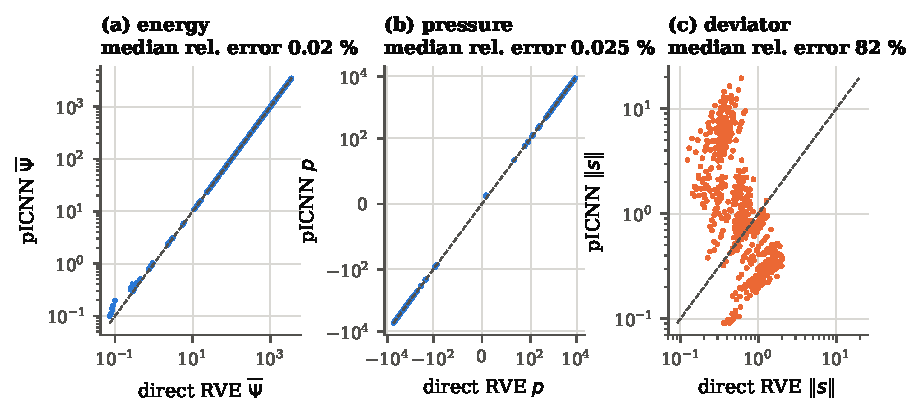
\includegraphics[width=\textwidth]{fig_parity.pdf}
\caption[Parity of the frozen pICNN against direct RVE solutions]{Parity of the frozen pICNN against direct RVE solutions on the Phase~7 test
states: (a) homogenized energy, (b) pressure $p=\tfrac13\operatorname{tr}\bm\sigma$
(symmetric logarithmic axes), (c) norm of the Cauchy stress deviator.}
\label{fig:parity}
\end{figure}

\paragraph{Inference.} Small training and test losses do not certify the model. The loss is dominated by the volumetric
part of the response, which the surrogate reproduces; the deviatoric part is practically not
constrained by it and is the actual weakness. The test losses being of the order of the
training loss shows that the model generalizes over the sampled states, not that it is accurate
in shear.

\section{Surrogate accuracy: two views of the same errors}\label{sec:accuracy}

\paragraph{The conventional view.} Energy and stress errors are commonly reported
as RMSE divided by the training RMS scales $s_\Psi$ and $s_P$. With this metric the
frozen checkpoint shows small errors (\cref{tab:nrmse}).

\begin{table}[htbp]
\centering\small
\caption{Normalized errors of the frozen checkpoint relative to the training scales.}
\label{tab:nrmse}
\begin{tabular}{@{}lrcc@{}}
\toprule
Evaluation set & Records & Energy NRMSE & Stress NRMSE\\
\midrule
Phase 7 independent, test split & 531 & $5.3\times10^{-4}$ & $1.0\times10^{-3}$\\
Fresh holdout, test split & 72 & $3.3\times10^{-4}$ & $8.0\times10^{-4}$\\
Fresh holdout, 30 benchmark cases & 30 & $4.3\times10^{-4}$ & $8.8\times10^{-4}$\\
\bottomrule
\end{tabular}
\end{table}

\paragraph{The physically separated view.} The Cauchy stress
$\bm\sigma=J^{-1}\Pstress\F^{\mathsf T}$ is split into the pressure
$p=\tfrac13\operatorname{tr}\bm\sigma$ and the deviator $\bm s=\bm\sigma-p\Iten$,
and the relative error of each part is evaluated record by record
(\code{figure\_sources\slash{}}, script \code{split\_metrics.py}). The picture changes
completely (\cref{tab:split}, \cref{fig:split}). Pressure is reproduced to a median
of $0.01$--$0.06\,\%$; only in the near-isochoric regime, where $p$ itself is small, does the median rise to $0.9\,\%$. The deviatoric stress, which governs shape
change and therefore everything the matrix does at nearly constant volume, has a
median error of $76$--$83\,\%$ (frozen) and $59$--$84\,\%$ (shear-adapted) outside
the expansion regime. In expansion states, where the deviator is small, the error
exceeds $1000\,\%$.

\begin{table}[htbp]
\centering\small
\caption[Median relative errors of pressure and deviatoric stress, Phase 7 test split]{Median relative errors of pressure and deviatoric stress, Phase~7 independent test split (531 records). RMS $\|\bm s\|$: size of the reference deviator.}
\label{tab:split}
\begin{tabular}{@{}lrcccc@{}}
\toprule
Regime & $n$ & RMS $p_\mathrm{ref}$ & RMS $\|\bm s_\mathrm{ref}\|$ & pressure & deviator\\
& & & & frozen & frozen / shear-adapted\\
\midrule
compression $J<0.7$ & 150 & 4559 & 1.19 & $0.014\,\%$ & $76\,\%$ / $79\,\%$\\
intermediate & 201 & 1927 & 0.67 & $0.055\,\%$ & $80\,\%$ / $62\,\%$\\
near-isochoric $|J-1|<0.02$ & 27 & 88 & 0.57 & $0.91\,\%$ & $80\,\%$ / $59\,\%$\\
expansion $J>1.4$ & 153 & 6774 & 0.36 & $0.029\,\%$ & $1557\,\%$ / $1422\,\%$\\
\midrule
all & 531 & 4528 & 0.79 & $0.025\,\%$ & $83\,\%$ / $84\,\%$\\
\bottomrule
\end{tabular}
\end{table}

\begin{figure}[htbp]
\centering
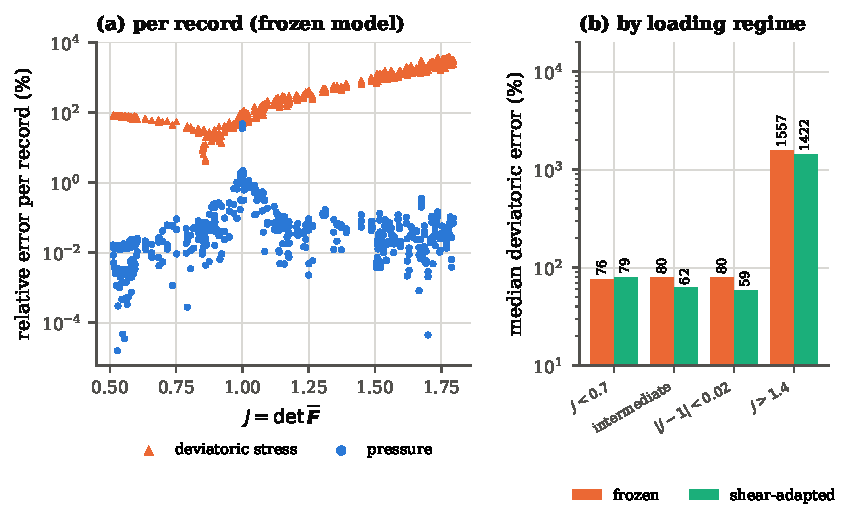
\includegraphics[width=\textwidth]{fig_split_errors.pdf}
\caption[Per-record relative errors of pressure and deviatoric stress against $J$]{(a) Per-record relative errors of pressure and deviatoric stress
against $J$ (frozen checkpoint). The two are separated by four orders of
magnitude. (b) Median deviatoric error by loading regime for both checkpoints.}
\label{fig:split}
\end{figure}

\paragraph{Inference.} The aggregate metric hides the problem: the same checkpoint has errors of order $10^{-4}$ in
pressure and of order $10^{-1}$--$10^{1}$ in the deviator. Acceptance of a surrogate for this
material must therefore be based on separate pressure and deviatoric errors. The fine-tune
does not remove the deviatoric error on the general test states (the difference between the two
checkpoints is within the scatter of the regimes), so it cannot be regarded as a general fix.

\section{Response along five loading paths}\label{sec:paths}

The test-set statistics of \cref{sec:accuracy} mix all loading modes. To see how
the error depends on the mode, the frozen surrogate was evaluated along the five
proportional loading paths of \cref{tab:paths}, from $0$ to $10\,\%$ amplitude and
for the three volume fractions, and compared with direct RVE solutions.

\begin{table}[htbp]
\centering\small
\caption[Proportional loading paths]{Proportional loading paths, amplitude $a\in[0,0.1]$. Direct RVE points:
solves of the earlier validation studies, i.e.\ volume-fraction map and shear-path check (E), and additional solves made for this comparison (N), both with
$h=0.22$ and integration order~10. At $a=0.10$ there is no direct point for uniaxial tension and compression at
$\vfrac=0.05$, and for simple shear only $\vfrac=0.05$ has one.}
\label{tab:paths}
\begin{tabular}{@{}llll@{}}
\toprule
Path & $\Fbar(a)$ & $\overline J$ at $a=0.1$ & Direct RVE points\\
\midrule
uniaxial tension & $\mathrm{diag}(1+a,1,1)$ & 1.100 & $a=0.05$ (E), $0.10$ (N)\\
uniaxial compression & $\mathrm{diag}(1-a,1,1)$ & 0.900 & $a=0.05$ (E), $0.10$ (N)\\
simple shear & $\Iten+a\,\bm e_1\otimes\bm e_2$ & 1.000 & $a=0.025,0.05,0.075$ (E), $0.10$ (N)\\
equibiaxial tension & $\mathrm{diag}(1+a,1+a,1)$ & 1.210 & $a=0.05,0.10$ (N)\\
volumetric expansion & $(1+a)^{1/3}\,\Iten$ & 1.100 & $a=0.05,0.10$ (N)\\
\bottomrule
\end{tabular}
\end{table}

\paragraph{Microscale fields.} \Cref{fig:rvefields} shows what the RVE computes for
two of these paths at $\vfrac=0.10$. Under uniaxial tension the response is
dominated by the volumetric part: the mean pressure is $549$, and the particle
perturbs it by only $-0.13$ to $+0.19$. The fluctuation $\bm w$ concentrates at the poles
of the particle along the loading axis, and the isochoric strain is amplified next
to the particle by a factor of about $2.6$ relative to the median value in the cell. Under simple
shear the pressure perturbation has the antisymmetric four-lobe pattern of a rigid
inclusion in shear, and the fluctuation is a factor of two smaller. The rigid
particle and its periodic images stiffen the matrix only through these local
deviatoric concentrations, which is why the effective shear modulus depends on
$\vfrac$ much more strongly than the bulk modulus.

\begin{figure}[htbp]
\centering
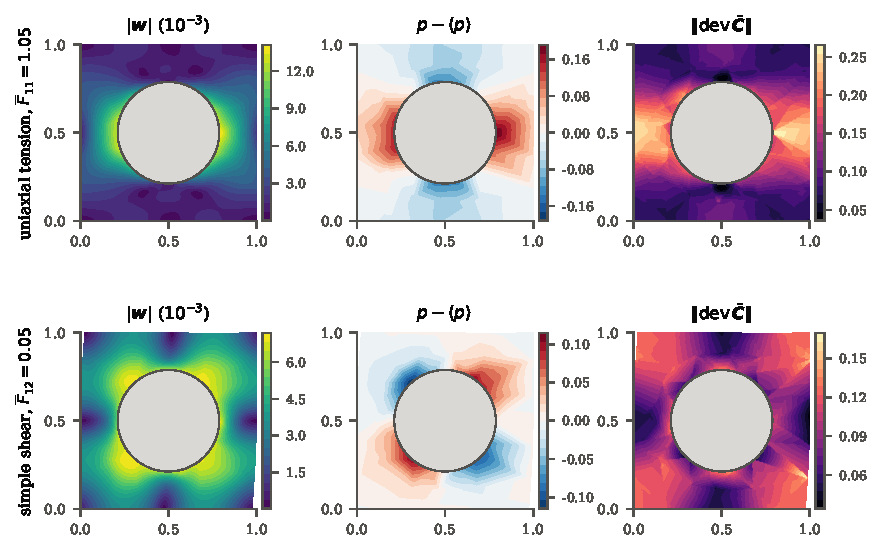
\includegraphics[width=\textwidth]{fig_rve_fields.pdf}
\caption[Direct RVE field solutions for $\vfrac=0.10$]{Direct RVE solutions for $\vfrac=0.10$ ($h=0.22$, order~10), section
$z=0.5$ through the particle centre, deformed configuration. Left: periodic
fluctuation $|\bm w|$. Centre: deviation of the pressure from its mean. Right:
isochoric strain measure $\|\mathrm{dev}\,\bar{\bm C}\|$. Grey: rigid particle.
Top: uniaxial tension $\overline F_{11}=1.05$. Bottom: simple shear $\overline F_{12}=0.05$.}
\label{fig:rvefields}
\end{figure}

\paragraph{Surrogate versus direct RVE.} \Cref{fig:loadpaths} shows the results.
For the four paths with a volume change, the surrogate follows the direct RVE
over the whole range: the relative stress error is between $10^{-4}$ and
$7.8\times10^{-3}$, and the largest energy error is $1.3\,\%$ ($\vfrac=0.10$,
$a=0.05$). Simple shear behaves differently. The surrogate is too stiff by $46\,\%$,
$55\,\%$ and $75\,\%$ for $\vfrac=0.02$, $0.05$ and $0.10$, and these errors are
the same at every amplitude from $2.5$ to $10\,\%$. The shear error is therefore a
wrong effective shear modulus, not a missing nonlinearity, in agreement with the
small-strain moduli of \cref{tab:moduli}. It grows with $\vfrac$ because the
surrogate also overestimates how strongly the shear stiffness depends on the volume
fraction (\cref{fig:vfdep}). From $\vfrac=0.02$ to $0.10$, the direct RVE stiffens by
$7.9\,\%$ in uniaxial tension and by $17\,\%$ in shear. Both values are close to
the Mori--Tanaka estimates of $8.9\,\%$ for $K$ and $22\,\%$ for $\mu$. The surrogate
reproduces the volumetric increase ($7.3\,\%$) but predicts $41\,\%$ in shear, a
factor of 2.4 too much.

\begin{figure}[htbp]
\centering
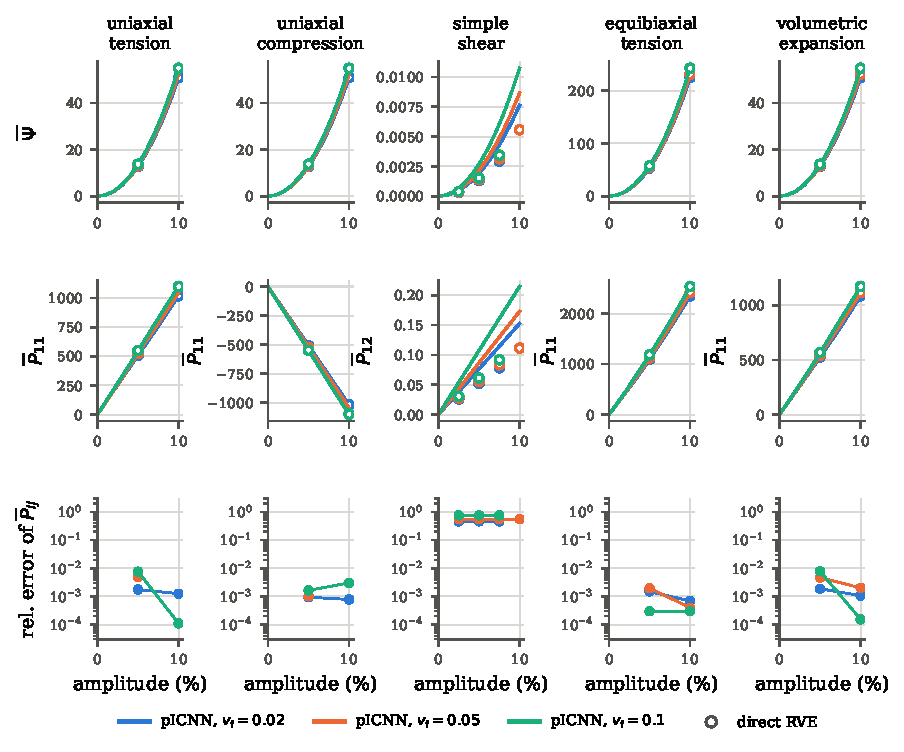
\includegraphics[width=\textwidth]{fig_load_paths.pdf}
\caption[Frozen pICNN and direct RVE along the five loading paths]{Frozen pICNN (lines) and direct RVE (circles) along the five loading paths of
\cref{tab:paths}. Rows: homogenized energy, active stress component, relative error
of that component. Simple shear is the only path without a volume change, and the
only one with a large error.}
\label{fig:loadpaths}
\end{figure}

\begin{figure}[htbp]
\centering
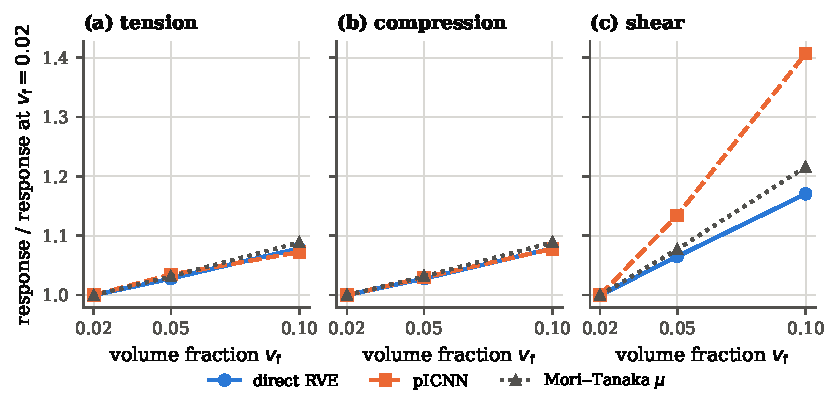
\includegraphics[width=\textwidth]{fig_vf_dependence.pdf}
\caption[Volume-fraction dependence at $5\,\%$ amplitude]{Volume-fraction dependence at $5\,\%$ amplitude, normalized by the value at
$\vfrac=0.02$: direct RVE, pICNN and the Mori--Tanaka ratio of the relevant modulus
(\cref{eq:mt}). (a) $\overline P_{11}$ in uniaxial tension, (b) $|\overline P_{11}|$ in uniaxial
compression, (c) $\overline P_{12}$ in simple shear.}
\label{fig:vfdep}
\end{figure}

\paragraph{Inference.} For loadings with a volume change the surrogate is accurate to within $0.8\,\%$ in stress and $1.3\,\%$ in energy
over the whole amplitude range and all volume fractions, and it follows the dependence on
$\vfrac$. In simple shear, the error is a constant factor at every amplitude, so it is an error of
the effective shear modulus, not of the nonlinearity. This directly motivates the separate
volumetric and isochoric energies of \cref{sec:proposed}.

\section{Diagnosis of the deviatoric error}\label{sec:diagnosis}

The evidence identifies one dominant cause and excludes several others.

\paragraph{Cause: the loss cannot see shear.} By \cref{eq:split}, volumetric and
deviatoric energies differ by the factor $K/\mu\approx10^4$ at comparable strains.
The combined Phase~6/7 dataset contains targeted states down to $J=0.51$ and up to $J=1.80$
(\cref{fig:coverage}). Of its 1671 records, only 90 ($5.4\,\%$) are near-isochoric ($|J-1|<0.02$), and only 111 ($6.6\,\%$) lie in the range $J\in[0.969,1.034]$ of the final $P_1$ states at $5\,\%$ stretch. (For the training split alone, 909 records, the counts are 54 and 63.) The
energy RMS of the combined dataset is $1127$ ($991$ for the training split), of which the isochoric part
$\approx\tfrac{\mu}{2}(\bar I_1-3)$ contributes an RMS of only $0.09$, about
$10^{-4}$. The loss \cref{eq:loss} normalizes by $s_\Psi=979$ and $s_P=2440$. The
decisive number follows directly: on the validation split, replacing the reference
stress by its volumetric part alone, that is \emph{deleting the entire deviatoric
response}, raises the stress loss by $8.1\times10^{-9}$. That is $1.5\,\%$ of the
validation stress loss actually reached ($5.3\times10^{-7}$). The $55\,\%$ error of $\overline P_{01}$ at $5\,\%$ simple shear contributes
only $\approx2\times10^{-11}$ to the stress loss of that record. To the optimizer, a model with
correct shear and a model with no shear are practically indistinguishable. The
relative-Frobenius tangent term has the same blindness, because $\|\Abar\|_F$ is
dominated by entries of order $K$. This is why, at $5\,\%$ shear, the full-tangent
error was only $1.0\,\%$ while the active component
$\partial\overline P_{01}/\partial\overline F_{01}$ was wrong by $55\,\%$
($1.731$ vs.\ $1.115$).

\paragraph{Aggravating factor: non-isochoric features.} The features
$I_1=J^{2/3}\bar I_1$ and $I_2=J^{4/3}\bar I_2$ change mostly with $J$ in the
training data. The same non-negative weights that fit the volumetric response
therefore also set the shear stiffness. The network has no separate degree of
freedom with which it could correct $\mu_{\mathrm{eff}}$ without disturbing $K$.

\paragraph{Excluded causes.} The direct-RVE labels are correct (Mori--Tanaka
agreement, P2-V5/V6). Stress and tangent are exact derivatives of the network
energy (S-V1). The reference state is exact (V2). An earlier feature-space
coverage audit placed the shear states in a \emph{dense} region of the
standardized feature space. This is consistent with the diagnosis: the shear
states are well covered in the features, but in a direction the loss ignores.

\begin{figure}[htbp]
\centering
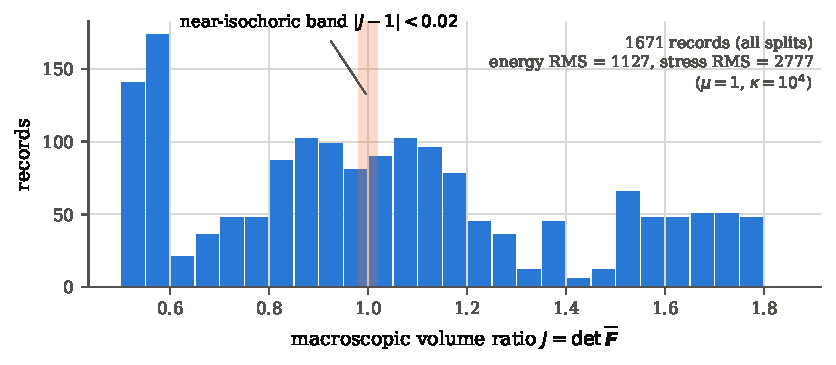
\includegraphics[width=\textwidth]{fig_training_coverage.pdf}
\caption[Determinant distribution of the 1671 records of the combined dataset]{Determinant distribution of the 1671 records of the combined Phase~6/7 dataset (training, validation and test splits). The targeted
compression and expansion tails dominate both the energy and the stress scales;
only $5.4\,\%$ of the records are near-isochoric.}
\label{fig:coverage}
\end{figure}

\section{Proposed surrogate improvements (not implemented)}\label{sec:proposed}

The diagnosis points to three changes. They are specified here for future work;
none of them was implemented or tested in this project.

\paragraph{Volumetric--isochoric energy.} In the present network, $I_1=J^{2/3}\bar I_1$
and $I_2=J^{4/3}\bar I_2$ enter through the same weights as $J$, so a single set of
parameters governs both the bulk and the shear response. An additive split
\begin{equation}
  \widehat\Psi(\F;\vfrac)=\Psi_{\mathrm{iso}}\bigl(\bar I_1,\bar I_2^{3/2};\vfrac\bigr)
  +\Psi_{\mathrm{vol}}(J;\vfrac),\qquad
  \bar I_1=J^{-2/3}I_1,\quad \bar I_2^{3/2}=J^{-2}I_2^{3/2},
  \label{eq:split-proposed}
\end{equation}
with one network per term separates the two. At $\F=\Iten$ the tangent of
\cref{eq:split-proposed} decomposes exactly into a volumetric part governed only by
$\Psi_{\mathrm{vol}}''(1)$ and a deviatoric part governed only by $\Psi_{\mathrm{iso}}$,
so $K_{\mathrm{eff}}$ and $\mu_{\mathrm{eff}}$ become independent quantities. Polyconvexity of
the complete energy follows from four conditions, all of which can be enforced by
construction:
\begin{enumerate}
  \item $\bar I_1$ and $\bar I_2^{3/2}$ are polyconvex functions of
        $\F$~\cite[Lemmas~2.1 and~2.2]{Hartmann2003};
  \item $\Psi_{\mathrm{iso}}$ is convex and non-decreasing in each of its two
        arguments (an ICNN with non-negative weights, as in \cref{sec:architecture}),
        so that the composition is polyconvex;
  \item $\Psi_{\mathrm{vol}}$ is convex in $J=\det\F$, and is therefore polyconvex;
        including $-\ln J$ as a feature with non-negative weight gives
        $\Psi_{\mathrm{vol}}\to\infty$ for $J\to0^{+}$;
  \item a sum of polyconvex functions is polyconvex.
\end{enumerate}
The normalization also separates. Because $\partial\bar I_1/\partial\F$ and
$\partial\bar I_2/\partial\F$ vanish at $\F=\Iten$, the isochoric part is stress-free
in the reference state by construction and needs only an energy offset. The
volumetric part is normalized by
$\Psi_{\mathrm{vol}}(J)-\Psi_{\mathrm{vol}}(1)-\Psi_{\mathrm{vol}}'(1)(J-1)$, which is affine in
$J$ and therefore preserves convexity and objectivity, as in \cref{eq:norm}.

\paragraph{Balanced loss.} The stress term of \cref{eq:loss} would be replaced by
separately normalized pressure and deviatoric terms,
\begin{equation}
  \mathcal L=w_\Psi\mathcal L_\Psi+w_p\,\frac{\langle(\hat p-p)^2\rangle}{s_p^2}
  +w_s\,\frac{\langle\Vert\operatorname{dev}\hat{\bm\sigma}-\operatorname{dev}\bm\sigma\Vert^2\rangle}{s_s^2}
  +w_A\mathcal L_A,
  \label{eq:loss-proposed}
\end{equation}
where $s_p$ and $s_s$ are the RMS values of the pressure and of the deviatoric-stress
norm in the training split. Both stress terms are then $O(1)$, so the deviatoric
response can no longer be neglected at the cost of $1.5\,\%$ of the loss, as found
above. The same scaling would apply to a split tangent term.

\paragraph{Sampling and metrics.} Training states would be sampled in the range of
$J$ consistent with $\kappa/\mu$ (the macroscopic runs stayed within
$J\in[0.969,1.034]$), with dense isochoric coverage instead of the present
$5.4\,\%$. Pressure error, deviatoric error, $K_{\mathrm{eff}}$ and $\mu_{\mathrm{eff}}$
(\cref{tab:split}) would be the primary acceptance measures, with the aggregate
NRMSE reported only alongside them. The split energy would also supply the separate
volumetric term that a mixed macroscopic formulation requires (\cref{sec:macro}).

\section{Shear fine-tuning}

The shear-adapted checkpoint was fitted on 18 of 33 additional simple-shear records
(6 more served for validation and 9 as a development test set), with the original data
replayed; the settings are in \cref{tab:trainconf}. The adaptation variants were compared on the
development set and the context holdout; the selected model was then evaluated, after it
had been frozen, on 12 new simple-shear cases generated afterwards. These cases use amplitudes
$\gamma=0.015$, $0.0325$, $0.0725$ and $0.0975$, all three volume fractions, and a
microstructure seed different from the adaptation data.

\begin{table}[htbp]
\centering\small
\caption{Final shear holdout (12 cases): mean relative errors.}
\label{tab:shear}
\begin{tabular}{@{}lccc@{}}
\toprule
Checkpoint & $\overline P_{01}$ & $\partial\overline P_{01}/\partial\overline F_{01}$ & energy\\
\midrule
frozen & $58.8\,\%$ & $58.7\,\%$ & $58.8\,\%$\\
shear-adapted & $40.1\,\%$ & $40.0\,\%$ & $40.1\,\%$\\
\bottomrule
\end{tabular}
\end{table}

The three errors are almost identical and independent of the amplitude: for the
frozen model, $58.7$--$58.8\,\%$ at every $\gamma$. This is the signature of a wrong
small-strain shear modulus rather than of a nonlinear misfit, in exact agreement
with \cref{tab:moduli}. Fine-tuning lowered $\mu_{\mathrm{eff}}$ by about $12\,\%$
and the error from $59\,\%$ to $40\,\%$ (\cref{fig:shear}). It did not, however,
improve the deviatoric error on the general Phase~7 states (median $83\,\%$ to
$84\,\%$, \cref{tab:split}). As the diagnosis predicts, the fine-tune moves the
shear modulus where shear data are added, but cannot fix a loss that is
insensitive to shear.

\begin{figure}[htbp]
\centering
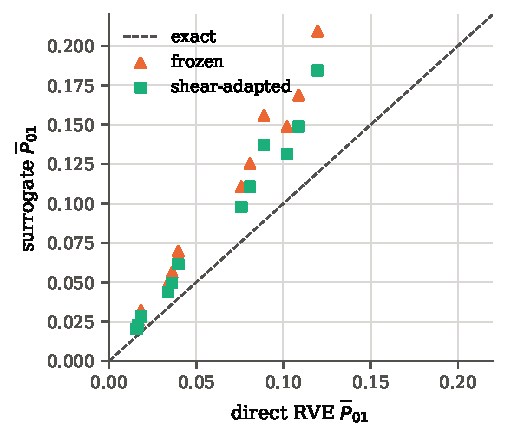
\includegraphics[width=0.48\textwidth]{fig_shear_holdout.pdf}
\caption[Final shear holdout: surrogate versus direct RVE]{Final shear holdout: surrogate versus direct RVE $\overline P_{01}$ for
12 unseen cases. Both checkpoints overestimate the shear stress by a nearly
constant factor.}
\label{fig:shear}
\end{figure}

\paragraph{Other evaluations of the frozen model, reinterpreted.} A loading-path
sweep (five modes, eleven amplitudes, 165 points) confirmed work conjugacy to
$4.6\times10^{-6}$ and tangent symmetry to $1.5\times10^{-15}$. An inverse design
of $\vfrac$ for target responses at $5\,\%$ loading succeeded for uniaxial
stretch (3/3 targets, $\le0.24\,\%$ error) and compression (3/3, $\le2.1\,\%$), but
not for simple shear: all shear targets lay outside the predicted range, and only one of three
reached the tolerance (at the lower bound of $\vfrac$). A sampled
acoustic-tensor screen (655 directions) found positive minima for both the
surrogate and the direct RVE. All these observations are consistent with the
diagnosis. Uniaxial states with $J\neq1$ are pressure-dominated and therefore well
predicted, whereas isochoric shear is not.

\paragraph{Inference.} The study shows that the shear error can be reduced only where shear data are added
($59\,\%\to40\,\%$), and that the remaining error is again a constant factor. This supports the
diagnosis that the loss, not the data volume or the architecture alone, limits the shear
accuracy. The fine-tuned checkpoint is a better shear model, but it is not a validated
substitute for the missing shear sensitivity of the loss.

% ======================================================================
\paragraph{Two other adaptation variants.}\label{sec:shearvariants}
Two further variants were trained from the same frozen checkpoint, with the same shear
data and original-data replay, before the full fine-tune was chosen. In the
\emph{context-only adapter} the invariant backbone is frozen and only the volume-fraction
context sub-network is trained (learning rate $10^{-5}$, seed $20261118$, extra weight $3$
on the low-amplitude shear tangent and on the identity tangent, selection restricted to a
loss of at most $2\,\%$ in original validation). On 12 new shear cases with amplitudes
disjoint from the adaptation data, it lowered the mean $\overline P_{01}$ error from
$58.8\,\%$ to $51.4\,\%$, against $40.1\,\%$ for the full fine-tune on the same cases;
these cases reuse the microstructure seed of the adaptation data. In the
\emph{shear-tangent calibration} (learning rate $2\times10^{-5}$, seed $20261117$) no
epoch improved on the starting model in the selection score, so the best epoch was
epoch~0 and the checkpoint remained identical to the frozen one. Only the full fine-tune, in which every
parameter may change, produced a clear reduction, and it is the variant used in the
following chapters. The reason why the other two failed was not investigated.

\section{Macroscopic application and volumetric locking}\label{sec:macro}

\paragraph{Results.} With the frozen surrogate ($\vfrac=0.05$), the clamped cube
of \cref{sec:macro-method} was solved with linear ($P_1$) and quadratic ($P_2$)
elements on three meshes (\cref{tab:macro}, \cref{fig:macro}). The $P_1$ runs
completed all 100 increments to $5\,\%$ stretch. The $P_2$ runs completed $0.5\,\%$ on
all meshes and $1\,\%$ on two of them; the $1\,\%$ run on the finest mesh stopped at
$0.70\,\%$ after 18 increments. All accepted states are converged to
$\|\bm R_\mathrm{free}\|<10^{-8}$ and orientation-preserving.

\begin{table}[htbp]
\centering\small
\caption[Macroscopic runs: energy, volume ratio and Newton effort]{Macroscopic runs: stored energy at the common stretch $\varepsilon=0.5\,\%$,
volume-ratio range and Newton effort. Free-uniaxial reference
$\tfrac32\mu_{\mathrm{eff}}\varepsilon^2$: $6.5\times10^{-5}$ with the pICNN
$\mu_{\mathrm{eff}}=1.731$.}
\label{tab:macro}
\begin{tabular}{@{}lrrrccr@{}}
\toprule
Order & $h$ & elements & DOFs & $\int\Psi\dd V$ at $0.5\,\%$ & $J_{\min}$ at $0.5\,\%$ & Newton it./step\\
\midrule
$P_1$ & 0.25 & 399 & 405 & $7.57\times10^{-3}$ & 0.99683 & 20.1\\
$P_1$ & 0.20 & 648 & 642 & $3.57\times10^{-3}$ & 0.99675 & 23.2\\
$P_1$ & 0.16 & 1818 & 1356 & $2.06\times10^{-3}$ & 0.99796 & 30.8\\
\midrule
$P_2$ & 0.25 & 399 & 2334 & $8.54\times10^{-5}$ & 0.99994 & 62.0\\
$P_2$ & 0.20 & 648 & 3759 & $8.36\times10^{-5}$ & 0.99994 & 81.4\\
$P_2$ & 0.16 & 1818 & 8928 & $8.29\times10^{-5}$ & 0.99985 & 101.3\\
\bottomrule
\end{tabular}
\end{table}

\begin{figure}[htbp]
\centering
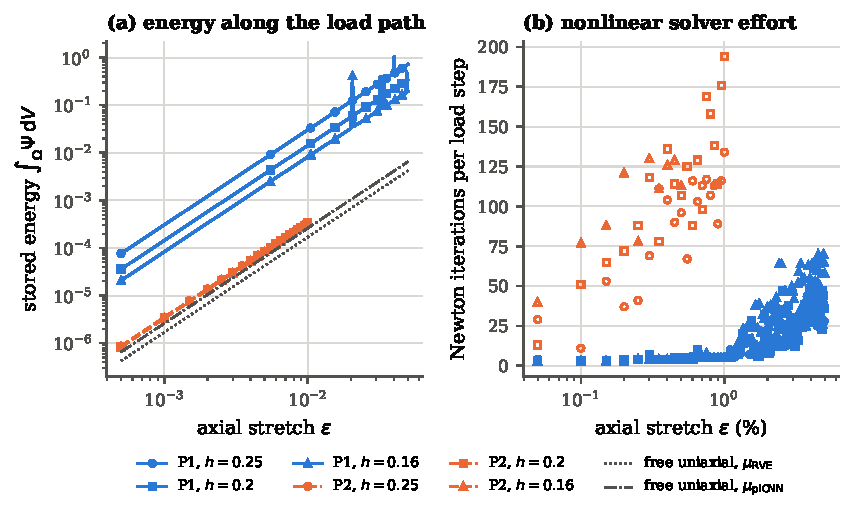
\includegraphics[width=\textwidth]{fig_macro_energy.pdf}
\caption[Macroscopic runs]{Macroscopic runs. (a) Stored energy along the load path. All curves grow
as $\varepsilon^2$, but the $P_1$ energies lie 25--89 times above the $P_2$ energies
and the analytical free-uniaxial estimates, and decrease strongly under
refinement; the $P_2$ energies change by $2.2\,\%$ and $0.8\,\%$. (b) Newton
iterations per load step.}
\label{fig:macro}
\end{figure}

\paragraph{Interpretation: the $P_1$ solution is locked.} Three independent
observations show that the $P_1$ energies are not physical.
\begin{enumerate}
  \item \emph{Magnitude.} At equal stretch, the $P_1$ energy exceeds the $P_2$ energy
        by factors of 89, 43 and 25 on the three meshes. The $P_2$ value is only
        $1.3$ times the analytical free-uniaxial estimate, a plausible stiffening
        for clamped ends.
  \item \emph{Mesh dependence.} The $P_1$ energy roughly halves with each refinement
        and converges very slowly towards the $P_2$ value. The $P_2$ value changes
        by only $2.2\,\%$ and $0.8\,\%$.
  \item \emph{Spurious volume change.} With an effective $K/\mu\approx10^4$, the
        $P_1$ solution still shows $J_{\min}=0.997$ at $0.5\,\%$ stretch, and
        $J\in[0.969,1.034]$ at $5\,\%$ on the coarsest mesh ($[0.969,1.030]$ and $[0.980,1.023]$ at $h=0.20$ and $0.16$). At $0.5\,\%$ the local volume changes are
        14--51 times larger than with $P_2$ (ratio of $1-J_{\min}$ on the three meshes).
\end{enumerate}
This is classical volumetric locking. Linear tetrahedra cannot represent
near-isochoric deformation fields~\cite{Simo1985,Zienkiewicz2013}. The RVE avoids
locking through its mixed $P_2/P_1$ formulation, but the macroscopic solver is
displacement-only. The $P_1$ result therefore demonstrates robust \emph{solver
integration} of the surrogate up to $5\,\%$, not a converged component response.

\paragraph{Interpretation: why $P_2$ is hard to drive.} The $P_2$ discretization is
far less locked, but its stiffness matrix inherits a condition number of
$3.3\times10^4$ (M-V0), of the order of the bulk-to-shear ratio $\kappa/\mu=10^4$. Starting from the affine predictor, the full
Newton step overshoots into inadmissible states ($J<0$ at some quadrature points).
The energy line search and the spectral shift then take many damped steps before
the final, quadratically convergent iterations; for example, the residuals
$9.1\times10^{-4}\to5.4\times10^{-5}\to2.5\times10^{-8}\to2.4\times10^{-13}$ close the
first increment at $h=0.25$. This explains the 62--137 iterations per increment. It
is a property of a displacement-only formulation of a nearly incompressible law,
not a defect of the surrogate.

\paragraph{Three distinct difficulties.} The macroscopic results combine three
effects with different causes and remedies.
\begin{enumerate}
  \item \emph{Volumetric locking} is a discretization error of the $P_1$
        interpolation: the displacement space cannot represent nearly
        volume-preserving, non-uniform fields. A uniform deformation is represented
        exactly (patch test V5), so the locking arises from the non-uniform field
        induced by the clamped faces. Evidence: the energy ratio, the mesh dependence
        and the spurious volume change listed above. Remedy: a mixed $u$--$p$ or
        $\bar{\bm F}$ formulation, or higher-order elements.
  \item \emph{Ill-conditioning} is an algebraic property: the stiffness matrix of a
        nearly incompressible material has eigenvalues spread by about $K/\mu$ (condition
        estimate $3.3\times10^4$, M-V0). It affects $P_1$ and $P_2$ alike and does not
        by itself make a solution inaccurate; with the sparse direct solver used here
        the residuals still reach $10^{-13}$. It would limit iterative linear solvers.
        Remedy: direct factorization or a block preconditioner.
  \item \emph{Inadmissible Newton states} are a nonlinear-solver issue: full steps from
        the affine predictor reach $J\le0$ at some quadrature points. The line search
        and spectral shift recover convergence at the cost of many iterations, and the
        finest $P_2$ run stopped at $0.70\,\%$. Remedy: better predictors, smaller
        increments or $J$-safeguarded updates.
\end{enumerate}
A mixed formulation addresses the first difficulty. It does not remove the other two
automatically: it leads to a saddle-point system, which requires an inf--sup stable
pair of spaces~\cite{Boffi2013} and a suitable linear solver, and its Newton iterations
still need globalization.

\paragraph{Consequences.} (i) A mixed $u$--$p$~\cite{Simo1985} or $\bar{\bm F}$~\cite{deSouzaNeto1996} macroscopic
formulation, which the project already implements at the RVE
level, is required for meaningful component responses. A mixed form of the type
\cref{eq:mixed} needs the volumetric part of the energy as a separate term; the
present single-network energy does not provide it, whereas the split energy
\cref{eq:split-proposed} does. The proposed surrogate change is therefore a
prerequisite for the proposed macroscopic formulation. (ii) The deviatoric bias of
\cref{sec:diagnosis} carries over to the macro scale: with the direct-RVE shear
modulus, the energy would be about $35\,\%$ lower ($1.124$ vs.\ $1.731$). (iii) The
shear-adapted checkpoint ran through the identical $P_1$ path. Its final energy
differs by only $0.65\,\%$, as expected for a locked, volumetrically dominated
solution.

\paragraph{Inference.} The surrogate can be integrated robustly into a finite-element solver (all $P_1$ runs reach $5\,\%$
stretch, all accepted states are converged and orientation-preserving), but the displacement-only
macroscopic model cannot give a converged component response for a nearly incompressible
material: the $P_1$ energies are locked, and the $P_2$ runs are limited by the nonlinear solver.
No statement about component-level accuracy of the surrogate is therefore possible from these
runs. They demonstrate integration and the required next step, a mixed formulation, but not
macroscopic accuracy.
